% Copyright 2004 by Till Tantau <tantau@users.sourceforge.net>.
%
% In principle, this file can be redistributed and/or modified under
% the terms of the GNU Public License, version 2.
%
% However, this file is supposed to be a template to be modified
% for your own needs. For this reason, if you use this file as a
% template and not specifically distribute it as part of a another
% package/program, I grant the extra permission to freely copy and
% modify this file as you see fit and even to delete this copyright
% notice. 

\documentclass{beamer}
\usepackage[utf8]{inputenc}



\usepackage{xspace}
\usepackage{pbox}
\usepackage[brazil]{babel}
\usepackage{xcolor}
\usepackage[alf]{abntex2cite}
\usepackage{url}
\definecolor{dark-gray}{gray}{0.20}
\definecolor{light-gray}{gray}{0.85}

\newcommand{\com}[1]{
\colorbox{light-gray}{\texttt{\pbox{\textwidth}{#1}}}
}

\newcommand{\cominline}[1]{
\colorbox{light-gray}{\texttt{\pbox{\textwidth}{#1}}}
}
% There are many different themes available for Beamer. A comprehensive
% list with examples is given here:
% http://deic.uab.es/~iblanes/beamer_gallery/index_by_theme.html
% You can uncomment the themes below if you would like to use a different
% one:
%\usetheme{AnnArbor}	%Legal
%\usetheme{Antibes}
%\usetheme{Bergen}
%\usetheme{Berkeley}
%\usetheme{Berlin}
%\usetheme{Boadilla} 	%Legal
%\usetheme{boxes}
\usetheme{CambridgeUS}	%Legal
%\usetheme{Copenhagen}	%Legal
%\usetheme{Darmstadt}
%\usetheme{default}
%\usetheme{Frankfurt}
%\usetheme{Goettingen}
%\usetheme{Hannover}
%\usetheme{Ilmenau}
%\usetheme{JuanLesPins}
%\usetheme{Luebeck}	%Legal
%\usetheme{Madrid}	%Legal
%\usetheme{Malmoe}	
%\usetheme{Marburg}
%\usetheme{Montpellier}
%\usetheme{PaloAlto}
%\usetheme{Pittsburgh}
%\usetheme{Rochester}
%\usetheme{Singapore}	%Legal
%\usetheme{Szeged}
%\usetheme{Warsaw}   


\title{Virtualização}

% A subtitle is optional and this may be deleted
%\subtitle{Optional Subtitle}

\author{Victor Canto\inst{1} Yuri Bergamo\inst{2}}
% - Give the names in the same order as the appear in the paper.
% - Use the \inst{?} command only if the authors have different
%   affiliation.
\institute[UNESP] % (optional, but mostly needed)
{
  Sistemas Distribuídos \newline \newline 
  \inst{1}%
  Bacharelado em Ciência da Computação \\
  
  \inst{2}% 
  Bacharelado em Sistemas de Informação \newline \newline
  Universidade Estadual Paulista “Júlio de Mesquita Filho” - UNESP
}
  
% - Use the \inst command only if there are several affiliations.
% - Keep it simple, no one is interested in your street address.

\date{22 de Dezembro de 2015.}
% - Either use conference name or its abbreviation.
% - Not really informative to the audience, more for people (including
%   yourself) who are reading the slides online

\subject{Theoretical Computer Science}
% This is only inserted into the PDF information catalog. Can be left
% out. 

% If you have a file called "university-logo-filename.xxx", where xxx
% is a graphic format that can be processed by latex or pdflatex,
% resp., then you can add a logo as follows:

% \pgfdeclareimage[height=0.5cm]{university-logo}{university-logo-filename}
% \logo{\pgfuseimage{university-logo}}

% Delete this, if you do not want the table of contents to pop up at
% the beginning of each subsection:


% Let's get started
\begin{document}

\begin{frame}
  \titlepage
\end{frame}

\begin{frame}{Sumário}
  \begin{itemize}
  \item
    O que é virtualização?
  
  \item
    Como funciona a virtualização?
   
  \item
    Virtualização X {\it Cloud}
   
  \item
    VMM/{\it Hypervisor}

  \item 
    Vantagens e desvantagens da virtualização.
  
  \item 
    Algumas ferramentas para virtualização.
  
  \item 
    Usos da virtualização.
    
   \item
    Dúvidas?
  
  \end{itemize}
\end{frame}



\begin{frame}{O que é virtualização?}
\begin{itemize}
 \item  A virtualização é o processo de criação de uma versão virtual, e não física, de algo. A virtualização pode ser aplicada a 
 computadores, SOs, dispositivos de armazenamento, aplicativos ou redes.
 \item A virtualização usa software para simular a existência de hardware e criar um sistema de computadores
virtual. Com isso, as empresas podem executar mais de um sistema virtual, e vários sistemas
operacionais e aplicativos, em um único servidor. Isso resulta em economias de escala e mais eficiência.
\end{itemize}
\end{frame}

\begin{frame}{Virtualização}
\begin{figure}[hbtp]
\centering
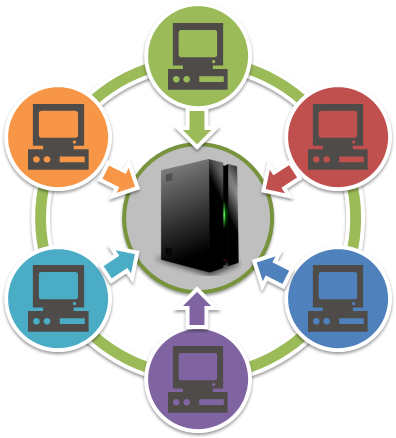
\includegraphics[width=6cm]{Images/virt.png}
\label{figRotulo}
\end{figure}
\end{frame}



\begin{frame}{Como funciona a virtualização?}
\begin{itemize}
\item Uma solução de virtualização é composta, essencialmente, por dois "protagonistas": o hospedeiro ({\it host}) e o hóspede ou convidado ({\it guest}).
\item As interações entre o hospedeiro e o hóspede variam de acordo com a solução.
\end{itemize}
\end{frame}

\begin{frame}{Virtualização X {\it Cloud}}
\begin{itemize}
  \item Computação em nuvem não é o mesmo que virtualização. Na verdade, computação em nuvem é algo
que você pode fazer usando virtualização. A computação em nuvem descreve o fornecimento de
recursos compartilhados de computação (software e/ou dados) sob demanda pela Internet. Quer ou não
esteja na nuvem, você poderá começar virtualizando seus servidores e, em seguida, passar para a
computação em nuvem para obter ainda mais agilidade.
\end{itemize}
\end{frame}

\begin{frame}{VMM/{\it Hypervisor}}
\begin{itemize}
 \item O {\it Hypervisor}, ou Monitor de Máquina Virtual (VMM), é uma camada de software entre o hardware e o sistema operacional.
 \item Fornece ao SO visitante, a abstração da máquina virtual.
 \item Além disso, controla o acesso do SO aos dispositivos {\it hardware}.
 \item Vale ressaltar que a sua execução é em modo privilegiado, pois ele executa e/ou simula instruções privilegiadas requisitadas pelo SO visitante. 
\end{itemize}
\end{frame}

\begin{frame}{VMM/{\it Hypervisor}}
\begin{figure}[hbtp]
\centering
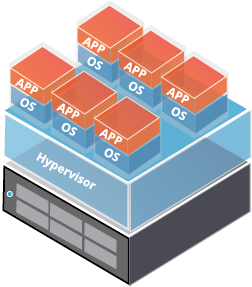
\includegraphics[width=6cm]{Images/hypervisor.png}
\label{figRotulo}
\end{figure}
\end{frame}


\begin{frame}{Tipos de virtualização - Virtualização Total}

\begin{itemize}
 \item A virtualização total tem por objetivo fornecer ao sistema operacional visitante uma réplica do hardware subjacente.
 \item O SO do hóspede trabalha como se de fato houvesse uma máquina física inteiramente à sua disposição
 \item Em uma outra definição, a máquina virtual simula todo o {\it hardware} para permitir que um SO hospedeiro seja executado de maneira isolada. 
 \item Uma limitação que pode ocorrer, é o risco de algumas solicitações do hóspede não serem atendidas da maneira esperada. 
 Isso acontece, por exemplo, quando o {\it hypervisor} não consegue lidar com determinada instrução privilegiada.

\end{itemize}
\end{frame}

\begin{frame}{Tipos de virtualização - Virtualização Total}
\begin{figure}[hbtp]
\centering
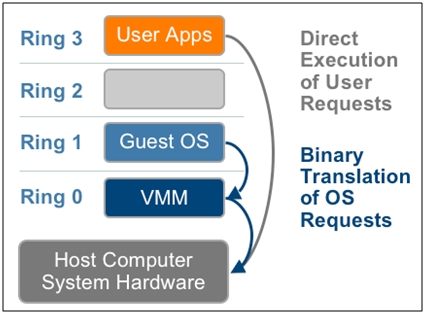
\includegraphics[width=9cm]{Images/TotalVirt.jpg}
\label{figRotulo}
\end{figure}
\end{frame}

\begin{frame}{Tipos de virtualização - Para-virtualização}

\begin{itemize}
 \item Uma alternativa à virtualização total.
 \item O SO da máquina virtual "possui" o conhecimento de que está rodando num ambiente virtualizado. 
 \item Neste método, o hóspede é modificado para recorrer ao hypervisor quando necessitar de qualquer instrução 
 privilegiada e não diretamente ao processador.
 \item Assim, o VMM não precisa interceptar estas solicitações e testá-las (tarefa que causa perda de desempenho), como acontece na virtualização total.
\end{itemize}
\end{frame}

\begin{frame}{Tipos de virtualização - Para-virtualização}
\begin{figure}[hbtp]
\centering
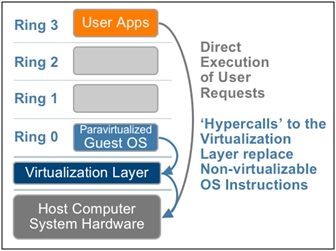
\includegraphics[width=9cm]{Images/paraVirt.jpg}
\label{figRotulo}
\end{figure}
\end{frame}

\begin{frame}{Tipos de virtualização - {\it Hardware}}
\begin{itemize}
\item Empresas como Intel (Intel VT) e AMD (AMD-V), as maiores fabricantes de processadores do mundo,
desenvolveram (e desenvolvem) tecnologias que possibilitam aos seus chips um trabalho
aprimorado em soluções de máquinas virtuais, especialmente no que diz respeito à
virtualização total.
\item Entre os recursos oferecidos por estas tecnologias está a capacidade de facilitar o
trabalho de fazer com que o processador funcione como um conjunto de chips, um para
cada máquina virtual em uso.

\end{itemize}
\end{frame}

\begin{frame}{Virtualização - Vantagens}
\begin{itemize}
\item Gerenciamento centralizado.
\item Instalações simplificadas.
\item Facilidade para a execução de backups.
\item Suporte e manutenção simplificados.
\item Acesso controlado a dados sensíveis e à propriedade intelectual mantendo-os seguros dentro do data center da empresa.
\item Independência de Hardware.
\item Disponibilização de novos servidores fica reduzida para alguns minutos.
\item Maior disponibilidade e mais fácil recuperação em caso de desastres.

\end{itemize}
\end{frame}
\begin{frame}{Virtualização - Vantagens}
\begin{itemize}
\item Economia de espaço físico.
\item Economia de energia elétrica utilizada em refrigeração e na alimentação dos servidores.
\item Melhor aproveitamento do {\it hardware}: com o compartilhamento do {\it hardware} entre as máquinas virtuais reduz-se a ociosidade
do equipamento.
\item Maior disponibilidade e mais fácil recuperação em caso de desastres.
\item Economia de espaço físico.
\item Melhor aproveitamento do {\it hardware}: com o compartilhamento do  {\it hardware} entre as máquinas virtuais reduz-se a ociosidade
do equipamento.
\item Economia de energia elétrica utilizada em refrigeração e na alimentação dos servidores.
\end{itemize}
\end{frame}

\begin{frame}{Virtualização - Desvantagens}
\begin{itemize}
\item Grande uso de espaço em disco, já que é preciso de todos os arquivos para cada sistema operacional instalado em cada máquina
virtual.
\item Dificuldade no acesso direto a {\it hardware}, como por exemplo placas específicas ou dispositivos USB
\item Grande consumo de memória RAM dado que cada máquina virtual vai ocupar uma área separada da mesma
\end{itemize}
\end{frame}

\begin{frame}{Virtualização - Desvantagens}
\begin{itemize}
\item Segurança: As máquinas virtuais podem ser menos seguras que as máquinas físicas justamente por causa do seu host. Este ponto
é interessante, pois se o sistema operacional hospedeiro tiver alguma vulnerabilidade, todas as máquinas virtuais que estão
hospedadas nessa máquina física estão vulneráveis.
\item Gerenciamento: Os ambientes virtuais necessitam ser instanciados, monitorados, configurados e salvos. Existem produtos que
fornecem essas soluções, mas esse é o campo no qual estão os maiores investimentos na área de virtualização, justamente por se
tratar de um dos maiores contra-tempos na implementação da virtualização.
\end{itemize}
\end{frame}


\begin{frame}{Algumas ferramentas de virtualização}
\begin{itemize}
\item {\it VMWare}
\item Xen
\item QEMU
\item VirtualBox
\end{itemize}
\end{frame}

\begin{frame}{Usos da Virtualização}
\begin{itemize}
 \item Consolidação de Servidores.
 \item Laboratórios de ensino.
 \item Desenvolvimento de Software.

\end{itemize}

 
\end{frame}


\begin{frame}{Dúvidas?}
\begin{figure}[hbtp]
\centering

\includegraphics[width=9cm]{Images/duvidas.png}
\label{figRotulo}
\end{figure}
\end{frame}

\end{document}




